\documentclass{extbook}[14pt]
\usepackage{multicol, enumerate, enumitem, hyperref, color, soul, setspace, parskip, fancyhdr, amssymb, amsthm, amsmath, bbm, latexsym, units, mathtools}
\everymath{\displaystyle}
\usepackage[headsep=0.5cm,headheight=0cm, left=1 in,right= 1 in,top= 1 in,bottom= 1 in]{geometry}
\usepackage{dashrule}  % Package to use the command below to create lines between items
\newcommand{\litem}[1]{\item #1

\rule{\textwidth}{0.4pt}}
\pagestyle{fancy}
\lhead{}
\chead{Answer Key for Progress Quiz 9 Version B}
\rhead{}
\lfoot{8590-6105}
\cfoot{}
\rfoot{Fall 2020}
\begin{document}
\textbf{This key should allow you to understand why you choose the option you did (beyond just getting a question right or wrong). \href{https://xronos.clas.ufl.edu/mac1105spring2020/courseDescriptionAndMisc/Exams/LearningFromResults}{More instructions on how to use this key can be found here}.}

\textbf{If you have a suggestion to make the keys better, \href{https://forms.gle/CZkbZmPbC9XALEE88}{please fill out the short survey here}.}

\textit{Note: This key is auto-generated and may contain issues and/or errors. The keys are reviewed after each exam to ensure grading is done accurately. If there are issues (like duplicate options), they are noted in the offline gradebook. The keys are a work-in-progress to give students as many resources to improve as possible.}

\rule{\textwidth}{0.4pt}

\begin{enumerate}\litem{
Describe the end behavior of the polynomial below.
\[ f(x) = 5(x + 8)^{3}(x - 8)^{8}(x + 6)^{5}(x - 6)^{5} \]

The solution is the graph below, which is option D.
\begin{center}
    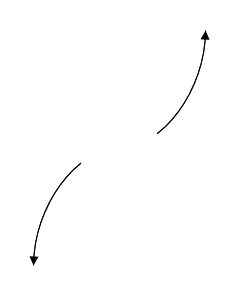
\includegraphics[width=0.3\textwidth]{../Figures/polyEndBehaviorDB.png}
\end{center}\begin{enumerate}[label=\Alph*.]
\begin{multicols}{2}
\item 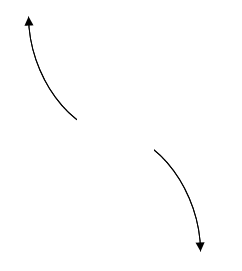
\includegraphics[width = 0.3\textwidth]{../Figures/polyEndBehaviorAB.png}
\item 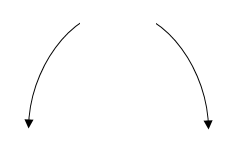
\includegraphics[width = 0.3\textwidth]{../Figures/polyEndBehaviorBB.png}
\item 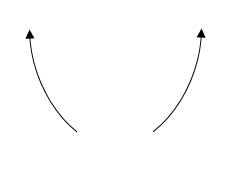
\includegraphics[width = 0.3\textwidth]{../Figures/polyEndBehaviorCB.png}
\item 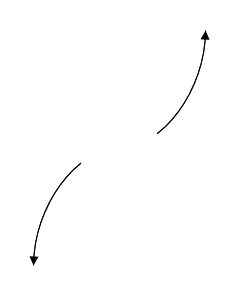
\includegraphics[width = 0.3\textwidth]{../Figures/polyEndBehaviorDB.png}
\end{multicols}\item None of the above.\end{enumerate}
\textbf{General Comment:} Remember that end behavior is determined by the leading coefficient AND whether the \textbf{sum} of the multiplicities is positive or negative.
}
\litem{
Which of the following equations \textit{could} be of the graph presented below?

\begin{center}
    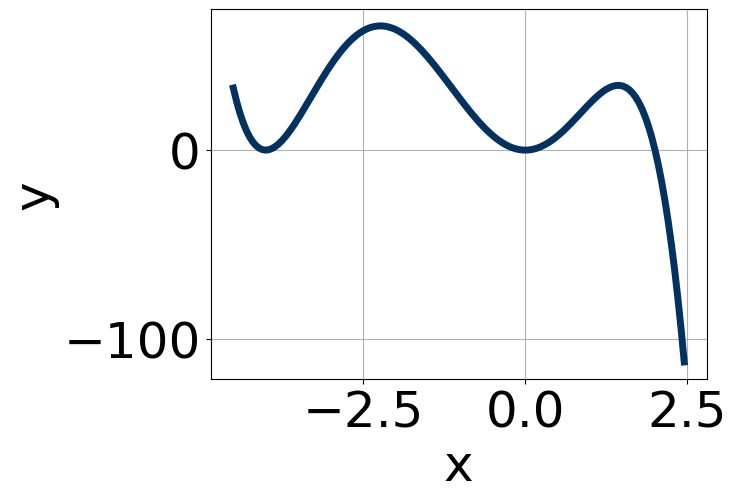
\includegraphics[width=0.5\textwidth]{../Figures/polyGraphToFunctionCopyB.png}
\end{center}




The solution is \( -3x^{5} (x - 1)^{6} (x + 4)^{11} \), which is option D.\begin{enumerate}[label=\Alph*.]
\item \( -20x^{8} (x - 1)^{4} (x + 4)^{5} \)

The factor $x$ should have an odd power.
\item \( 14x^{5} (x - 1)^{4} (x + 4)^{4} \)

The factor $(x + 4)$ should have an odd power and the leading coefficient should be the opposite sign.
\item \( -7x^{6} (x - 1)^{5} (x + 4)^{9} \)

The factor $1$ should have an even power and the factor $0$ should have an odd power.
\item \( -3x^{5} (x - 1)^{6} (x + 4)^{11} \)

* This is the correct option.
\item \( 20x^{7} (x - 1)^{10} (x + 4)^{11} \)

This corresponds to the leading coefficient being the opposite value than it should be.
\end{enumerate}

\textbf{General Comment:} General Comments: Draw the x-axis to determine which zeros are touching (and so have even multiplicity) or cross (and have odd multiplicity).
}
\litem{
Construct the lowest-degree polynomial given the zeros below. Then, choose the intervals that contain the coefficients of the polynomial in the form $ax^3+bx^2+cx+d$.
\[ \frac{7}{2}, \frac{-4}{5}, \text{ and } -1 \]

The solution is \( 10x^{3} -17 x^{2} -55 x -28 \), which is option E.\begin{enumerate}[label=\Alph*.]
\item \( a \in [8, 21], b \in [14, 22], c \in [-56, -48], \text{ and } d \in [21, 32] \)

$10x^{3} +17 x^{2} -55 x + 28$, which corresponds to multiplying out $(2x + 7)(5x -4)(x -1)$.
\item \( a \in [8, 21], b \in [32, 42], c \in [-1, 9], \text{ and } d \in [-30, -24] \)

$10x^{3} +37 x^{2} -x -28$, which corresponds to multiplying out $(2x + 7)(5x -4)(x + 1)$.
\item \( a \in [8, 21], b \in [45, 61], c \in [65, 76], \text{ and } d \in [21, 32] \)

$10x^{3} +53 x^{2} +71 x + 28$, which corresponds to multiplying out $(2x + 7)(5x + 4)(x + 1)$.
\item \( a \in [8, 21], b \in [-17, -10], c \in [-56, -48], \text{ and } d \in [21, 32] \)

$10x^{3} -17 x^{2} -55 x + 28$, which corresponds to multiplying everything correctly except the constant term.
\item \( a \in [8, 21], b \in [-17, -10], c \in [-56, -48], \text{ and } d \in [-30, -24] \)

* $10x^{3} -17 x^{2} -55 x -28$, which is the correct option.
\end{enumerate}

\textbf{General Comment:} To construct the lowest-degree polynomial, you want to multiply out $(2x -7)(5x + 4)(x + 1)$
}
\litem{
Construct the lowest-degree polynomial given the zeros below. Then, choose the intervals that contain the coefficients of the polynomial in the form $ax^3+bx^2+cx+d$.
\[ \frac{4}{3}, \frac{-4}{5}, \text{ and } \frac{-5}{3} \]

The solution is \( 45x^{3} +51 x^{2} -88 x -80 \), which is option B.\begin{enumerate}[label=\Alph*.]
\item \( a \in [38, 47], b \in [-53, -46], c \in [-95, -81], \text{ and } d \in [75, 85] \)

$45x^{3} -51 x^{2} -88 x + 80$, which corresponds to multiplying out $(3x + 4)(5x -4)(3x -5)$.
\item \( a \in [38, 47], b \in [46, 59], c \in [-95, -81], \text{ and } d \in [-82, -72] \)

* $45x^{3} +51 x^{2} -88 x -80$, which is the correct option.
\item \( a \in [38, 47], b \in [46, 59], c \in [-95, -81], \text{ and } d \in [75, 85] \)

$45x^{3} +51 x^{2} -88 x + 80$, which corresponds to multiplying everything correctly except the constant term.
\item \( a \in [38, 47], b \in [96, 104], c \in [-8, 0], \text{ and } d \in [-82, -72] \)

$45x^{3} +99 x^{2} -8 x -80$, which corresponds to multiplying out $(3x + 4)(5x -4)(3x + 5)$.
\item \( a \in [38, 47], b \in [170, 174], c \in [208, 212], \text{ and } d \in [75, 85] \)

$45x^{3} +171 x^{2} +208 x + 80$, which corresponds to multiplying out $(3x + 4)(5x + 4)(3x + 5)$.
\end{enumerate}

\textbf{General Comment:} To construct the lowest-degree polynomial, you want to multiply out $(3x -4)(5x + 4)(3x + 5)$
}
\litem{
Construct the lowest-degree polynomial given the zeros below. Then, choose the intervals that contain the coefficients of the polynomial in the form $x^3+bx^2+cx+d$.
\[ 3 + 2 i \text{ and } 4 \]

The solution is \( x^{3} -10 x^{2} +37 x -52 \), which is option B.\begin{enumerate}[label=\Alph*.]
\item \( b \in [-3, 3], c \in [-7.24, -6.71], \text{ and } d \in [12, 18] \)

$x^{3} + x^{2} -7 x + 12$, which corresponds to multiplying out $(x -3)(x -4)$.
\item \( b \in [-17, -6], c \in [35.65, 38.84], \text{ and } d \in [-55, -51] \)

* $x^{3} -10 x^{2} +37 x -52$, which is the correct option.
\item \( b \in [-3, 3], c \in [-6.62, -5.73], \text{ and } d \in [0, 11] \)

$x^{3} + x^{2} -6 x + 8$, which corresponds to multiplying out $(x -2)(x -4)$.
\item \( b \in [9, 11], c \in [35.65, 38.84], \text{ and } d \in [47, 55] \)

$x^{3} +10 x^{2} +37 x + 52$, which corresponds to multiplying out $(x-(3 + 2 i))(x-(3 - 2 i))(x + 4)$.
\item \( \text{None of the above.} \)

This corresponds to making an unanticipated error or not understanding how to use nonreal complex numbers to create the lowest-degree polynomial. If you chose this and are not sure what you did wrong, please contact the coordinator for help.
\end{enumerate}

\textbf{General Comment:} Remember that the conjugate of $a+bi$ is $a-bi$. Since these zeros always come in pairs, we need to multiply out $(x-(3 + 2 i))(x-(3 - 2 i))(x-(4))$.
}
\litem{
Construct the lowest-degree polynomial given the zeros below. Then, choose the intervals that contain the coefficients of the polynomial in the form $x^3+bx^2+cx+d$.
\[ -3 - 2 i \text{ and } -1 \]

The solution is \( x^{3} +7 x^{2} +19 x + 13 \), which is option D.\begin{enumerate}[label=\Alph*.]
\item \( b \in [-1.4, 1.6], c \in [2.69, 3.9], \text{ and } d \in [0.87, 2.86] \)

$x^{3} + x^{2} +3 x + 2$, which corresponds to multiplying out $(x + 2)(x + 1)$.
\item \( b \in [-1.4, 1.6], c \in [3.53, 4.78], \text{ and } d \in [2.66, 3.65] \)

$x^{3} + x^{2} +4 x + 3$, which corresponds to multiplying out $(x + 3)(x + 1)$.
\item \( b \in [-7.8, -5.8], c \in [18.72, 19.42], \text{ and } d \in [-13.71, -12.62] \)

$x^{3} -7 x^{2} +19 x -13$, which corresponds to multiplying out $(x-(-3 - 2 i))(x-(-3 + 2 i))(x -1)$.
\item \( b \in [3.5, 10.6], c \in [18.72, 19.42], \text{ and } d \in [10, 13.23] \)

* $x^{3} +7 x^{2} +19 x + 13$, which is the correct option.
\item \( \text{None of the above.} \)

This corresponds to making an unanticipated error or not understanding how to use nonreal complex numbers to create the lowest-degree polynomial. If you chose this and are not sure what you did wrong, please contact the coordinator for help.
\end{enumerate}

\textbf{General Comment:} Remember that the conjugate of $a+bi$ is $a-bi$. Since these zeros always come in pairs, we need to multiply out $(x-(-3 - 2 i))(x-(-3 + 2 i))(x-(-1))$.
}
\litem{
Describe the zero behavior of the zero $x = -5$ of the polynomial below.
\[ f(x) = 4(x + 5)^{6}(x - 5)^{11}(x - 6)^{6}(x + 6)^{9} \]

The solution is the graph below, which is option B.
\begin{center}
    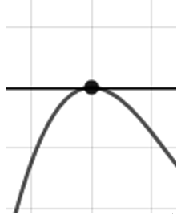
\includegraphics[width=0.3\textwidth]{../Figures/polyZeroBehaviorCopyBB.png}
\end{center}\begin{enumerate}[label=\Alph*.]
\begin{multicols}{2}
\item 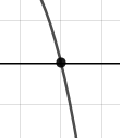
\includegraphics[width = 0.3\textwidth]{../Figures/polyZeroBehaviorCopyAB.png}
\item 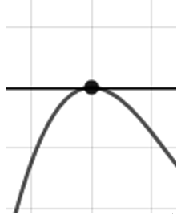
\includegraphics[width = 0.3\textwidth]{../Figures/polyZeroBehaviorCopyBB.png}
\item 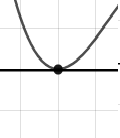
\includegraphics[width = 0.3\textwidth]{../Figures/polyZeroBehaviorCopyCB.png}
\item 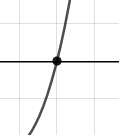
\includegraphics[width = 0.3\textwidth]{../Figures/polyZeroBehaviorCopyDB.png}
\end{multicols}\item None of the above.\end{enumerate}
\textbf{General Comment:} You will need to sketch the entire graph, then zoom in on the zero the question asks about.
}
\litem{
Describe the end behavior of the polynomial below.
\[ f(x) = -3(x - 9)^{5}(x + 9)^{6}(x - 3)^{4}(x + 3)^{6} \]

The solution is the graph below, which is option A.
\begin{center}
    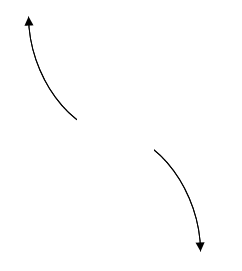
\includegraphics[width=0.3\textwidth]{../Figures/polyEndBehaviorCopyAB.png}
\end{center}\begin{enumerate}[label=\Alph*.]
\begin{multicols}{2}
\item 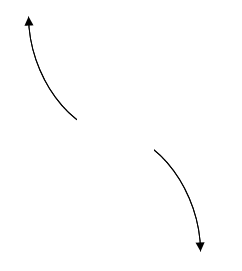
\includegraphics[width = 0.3\textwidth]{../Figures/polyEndBehaviorCopyAB.png}
\item 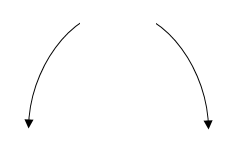
\includegraphics[width = 0.3\textwidth]{../Figures/polyEndBehaviorCopyBB.png}
\item 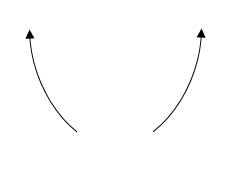
\includegraphics[width = 0.3\textwidth]{../Figures/polyEndBehaviorCopyCB.png}
\item 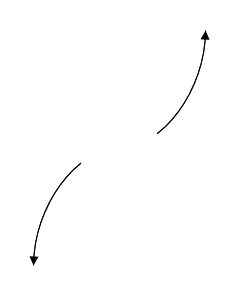
\includegraphics[width = 0.3\textwidth]{../Figures/polyEndBehaviorCopyDB.png}
\end{multicols}\item None of the above.\end{enumerate}
\textbf{General Comment:} Remember that end behavior is determined by the leading coefficient AND whether the \textbf{sum} of the multiplicities is positive or negative.
}
\litem{
Which of the following equations \textit{could} be of the graph presented below?

\begin{center}
    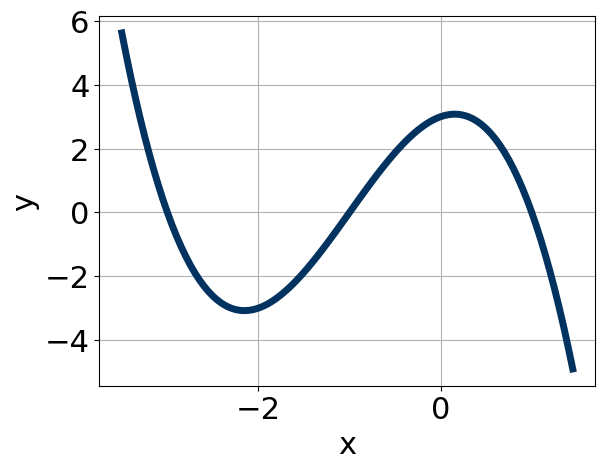
\includegraphics[width=0.5\textwidth]{../Figures/polyGraphToFunctionB.png}
\end{center}




The solution is \( -5(x + 1)^{4} (x + 2)^{6} (x - 2)^{4} \), which is option D.\begin{enumerate}[label=\Alph*.]
\item \( -3(x + 1)^{10} (x + 2)^{8} (x - 2)^{11} \)

The factor $(x - 2)$ should have an even power.
\item \( -19(x + 1)^{4} (x + 2)^{9} (x - 2)^{9} \)

The factors $(x + 2)$ and $(x - 2)$ should both have even powers.
\item \( 15(x + 1)^{4} (x + 2)^{10} (x - 2)^{9} \)

The factor $(x - 2)$ should have an even power and the leading coefficient should be the opposite sign.
\item \( -5(x + 1)^{4} (x + 2)^{6} (x - 2)^{4} \)

* This is the correct option.
\item \( 15(x + 1)^{4} (x + 2)^{8} (x - 2)^{4} \)

This corresponds to the leading coefficient being the opposite value than it should be.
\end{enumerate}

\textbf{General Comment:} General Comments: Draw the x-axis to determine which zeros are touching (and so have even multiplicity) or cross (and have odd multiplicity).
}
\litem{
Describe the zero behavior of the zero $x = 2$ of the polynomial below.
\[ f(x) = 8(x - 7)^{6}(x + 7)^{3}(x - 2)^{6}(x + 2)^{3} \]

The solution is the graph below, which is option C.
\begin{center}
    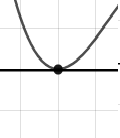
\includegraphics[width=0.3\textwidth]{../Figures/polyZeroBehaviorCB.png}
\end{center}\begin{enumerate}[label=\Alph*.]
\begin{multicols}{2}
\item 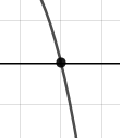
\includegraphics[width = 0.3\textwidth]{../Figures/polyZeroBehaviorAB.png}
\item 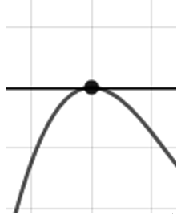
\includegraphics[width = 0.3\textwidth]{../Figures/polyZeroBehaviorBB.png}
\item 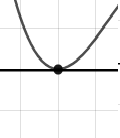
\includegraphics[width = 0.3\textwidth]{../Figures/polyZeroBehaviorCB.png}
\item 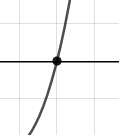
\includegraphics[width = 0.3\textwidth]{../Figures/polyZeroBehaviorDB.png}
\end{multicols}\item None of the above.\end{enumerate}
\textbf{General Comment:} You will need to sketch the entire graph, then zoom in on the zero the question asks about.
}
\end{enumerate}

\end{document}